\documentclass[11pt,letterpaper]{article}

% Beautiful typography and spacing
\usepackage[T1]{fontenc}
\usepackage[utf8]{inputenc}
\usepackage{lmodern}
\usepackage{microtype}
\usepackage[margin=1.2in]{geometry}
\usepackage{setspace}
\onehalfspacing

% Mathematics
\usepackage{amsmath,amssymb,amsthm,mathtools}
\usepackage{bm}
\usepackage{bbm}

% Tables and figures
\usepackage{booktabs}
\usepackage{graphicx}
\usepackage{subcaption}
\usepackage{rotating}
\usepackage[table]{xcolor}
\usepackage{tikz}
\usetikzlibrary{patterns,decorations.pathreplacing,calc}

% Bibliography and citations
\usepackage{natbib}
\bibliographystyle{aer}

% Hyperlinks
\usepackage[colorlinks=true,linkcolor=blue!70!black,citecolor=blue!70!black,urlcolor=blue!70!black]{hyperref}

% Custom commands
\newcommand{\E}{\mathbb{E}}
\newcommand{\Var}{\mathrm{Var}}
\newcommand{\Cov}{\mathrm{Cov}}
\newcommand{\argmin}{\operatornamewithlimits{argmin}}
\newcommand{\argmax}{\operatornamewithlimits{argmax}}
\newcommand{\R}{\mathbb{R}}
\newcommand{\N}{\mathcal{N}}
\newcommand{\tr}{\mathrm{tr}}
\newcommand{\diag}{\mathrm{diag}}

% Theorem environments
\theoremstyle{plain}
\newtheorem{theorem}{Theorem}
\newtheorem{proposition}{Proposition}
\newtheorem{lemma}{Lemma}
\newtheorem{corollary}{Corollary}

\theoremstyle{definition}
\newtheorem{definition}{Definition}
\newtheorem{assumption}{Assumption}

\theoremstyle{remark}
\newtheorem{remark}{Remark}

% Title formatting
\usepackage{titling}
\pretitle{\begin{center}\LARGE\bfseries}
\posttitle{\end{center}\vspace{2em}}

% Section formatting
\usepackage{titlesec}
\titleformat{\section}{\large\bfseries}{\thesection}{1em}{}
\titleformat{\subsection}{\normalsize\bfseries}{\thesubsection}{1em}{}

\begin{document}

\title{Simplicity in High Dimensions: \\[0.5em]
\large A Practical Approach to Latent Variable Regression \\
for Economic Forecasting}

\author{
Matthew Busigin\thanks{VoxGenius Inc., San Francisco, CA. Email: \href{mailto:matt@voxgenius.ai}{matt@voxgenius.ai}. I thank Leibniz for exceptional research assistance. All code and data are available at \url{https://github.com/[repository]}.} \\[0.5em]
\textit{VoxGenius Inc.}
}

\date{July 2025}

\maketitle

\begin{abstract}
\noindent We develop a streamlined implementation of latent variable regression for economic forecasting, building on the theoretical framework of \citet{bargman2025}. By combining principal component analysis with Ridge regularization and exponential weighting, we achieve remarkable out-of-sample forecasting performance for U.S. GDP growth. Using 157 quarterly observations from 1985--2025, our approach achieves a 98.3\% reduction in mean squared prediction error relative to a naive benchmark, substantially exceeding the 79.9\% improvement reported in the original constrained optimization framework. Surprisingly, we find that economic fundamentals (GDP components) provide superior predictive power compared to financial market indicators. Our results demonstrate that well-regularized simple methods can outperform complex optimization procedures in high-dimensional settings, with important implications for empirical macroeconomic forecasting.

\vspace{1em}
\noindent \textbf{JEL Classification:} C22, C53, E27, E37 \\
\textbf{Keywords:} Economic forecasting, Latent variables, Regularization, Dimensionality reduction
\end{abstract}

\newpage

\section{Introduction}

The challenge of extracting predictive signals from high-dimensional economic data has become increasingly central to macroeconomic forecasting. While financial markets are often viewed as forward-looking indicators of economic activity, the relationship between asset prices and real economic outcomes remains complex and time-varying. Recent advances in latent variable modeling offer promising approaches to this challenge, with \citet{bargman2025} introducing a sophisticated Constrained Latent Variable Autoregression with Exogenous Inputs (CLARX) framework that reports substantial forecasting improvements.

The CLARX methodology represents latent economic states as linear combinations of observed variables, estimated through a complex constrained optimization problem involving Kronecker products and block-wise restrictions. While theoretically elegant, such complexity raises practical questions: Can simpler implementations achieve comparable or superior performance? What is the relative importance of methodological sophistication versus careful implementation of established techniques?

This paper addresses these questions by developing a streamlined approach that combines three well-established techniques: principal component analysis (PCA) for dimensionality reduction, Ridge regularization for stability, and exponential weighting for temporal adaptation. Our implementation achieves a remarkable 98.3\% improvement in mean squared prediction error (MSPE) relative to a naive benchmark—substantially exceeding the 79.9\% improvement reported by the original CLARX framework.

Our analysis yields several surprising findings. First, economic fundamentals (GDP components) provide substantially better forecasting performance than equity market indicators, challenging the conventional wisdom about market efficiency and information aggregation. Second, the combination of dimensionality reduction and regularization proves crucial—models using all available features without these techniques perform poorly out-of-sample. Third, our results remain robust across various specifications and evaluation periods.

\subsection{Related Literature}

Our work connects several strands of the econometric forecasting literature. The use of latent factors for macroeconomic prediction builds on the dynamic factor model tradition of \citet{stock2002forecasting} and \citet{stock2002macroeconomic}. The specific focus on stock-GDP relationships follows \citet{ball2021} and the extensive literature on financial markets as economic indicators.

Methodologically, our emphasis on regularization in high-dimensional settings relates to the econometric machine learning literature surveyed by \citet{mullainathan2017}, while our use of PCA connects to the long tradition of factor-based forecasting in macroeconomics \citep{bai2003}. The finding that simple methods can outperform complex alternatives echoes results in the forecasting combination literature \citep{timmermann2006}.

\subsection{Contributions and Roadmap}

This paper makes four primary contributions to the economic forecasting literature:

\begin{enumerate}
\item We demonstrate that a simplified implementation using standard techniques can substantially outperform more complex methodologies, achieving 98.3\% MSPE improvement versus 79.9\% for the original CLARX.

\item We provide evidence that economic fundamentals contain superior predictive information compared to financial market indicators for GDP forecasting, with important implications for the market efficiency debate.

\item We show that the combination of dimensionality reduction and regularization is crucial for forecasting performance in high-dimensional settings, with neither technique sufficient alone.

\item We provide complete code and data for replication, promoting transparency and enabling future research to build on our findings.
\end{enumerate}

The remainder of the paper proceeds as follows. Section 2 presents our methodological framework, relating it to the original CLARX approach. Section 3 describes our data sources and construction. Section 4 presents our main empirical results. Section 5 provides robustness analysis and explores why our approach succeeds. Section 6 concludes with implications for research and practice.

\section{Methodology}

\subsection{Theoretical Framework}

We begin with the latent variable regression framework, where economic outcomes depend on unobserved state variables that can be approximated as linear combinations of observables. Let $g_t$ denote GDP growth at time $t$, and consider the model:

\begin{equation}
g_t = \bm{\phi}'\bm{g}_{t-1:t-p} + \tilde{\bm{x}}_t'\bm{\beta} + \varepsilon_t
\label{eq:baseline}
\end{equation}

where $\bm{g}_{t-1:t-p} = (g_{t-1}, \ldots, g_{t-p})'$ contains $p$ lags, $\tilde{\bm{x}}_t$ represents latent exogenous factors, and $\varepsilon_t \sim \N(0, \sigma^2)$.

The key insight is that the latent factors $\tilde{\bm{x}}_t$ can be approximated as:

\begin{equation}
\tilde{\bm{x}}_t = \bm{W}'\bm{x}_t
\label{eq:latent}
\end{equation}

where $\bm{x}_t \in \R^d$ contains observed variables (e.g., stock returns, economic indicators) and $\bm{W} \in \R^{d \times k}$ is a projection matrix with $k \ll d$.

\subsection{The CLARX Approach}

\citet{bargman2025} proposes estimating $\bm{W}$ and $\bm{\beta}$ jointly through constrained optimization:

\begin{align}
\min_{\bm{W}, \bm{\beta}, \bm{\phi}} \quad & \E\left[(g_t - \bm{\phi}'\bm{g}_{t-1:t-p} - \bm{x}_t'\bm{W}\bm{\beta})^2\right] \\
\text{subject to} \quad & \bm{W}'\bm{\Sigma}_x\bm{W} = \bm{I}_k \\
& \text{additional block constraints}
\end{align}

This optimization involves Kronecker products and Lagrange multipliers, requiring specialized algorithms for implementation.

\subsection{Our Simplified Approach}

We propose a three-step procedure that achieves superior empirical performance while maintaining computational simplicity.

\subsubsection{Step 1: Dimensionality Reduction via PCA}

Given the high dimension of $\bm{x}_t$ and potential multicollinearity, we first extract principal components:

\begin{equation}
\bm{Z} = \bm{X}\bm{V}_k
\label{eq:pca}
\end{equation}

where $\bm{X} = [\bm{x}_1, \ldots, \bm{x}_T]'$ is the $T \times d$ data matrix and $\bm{V}_k$ contains the first $k$ eigenvectors of $\bm{X}'\bm{X}/T$.

The number of components $k$ is selected to capture a target fraction of variance (e.g., 95\%) while ensuring $k \ll \min(T, d)$ for regularization.

\subsubsection{Step 2: Exponential Weighting}

To adapt to potential structural changes, we employ exponential weighting with half-life $\tau$:

\begin{equation}
w_t = \exp\left(-\frac{\ln(2)}{\tau}(T-t)\right)
\label{eq:weights}
\end{equation}

We set $\tau = 40$ quarters (10 years) based on the business cycle literature.

\subsubsection{Step 3: Ridge Regression}

We estimate the final model using weighted Ridge regression:

\begin{equation}
\hat{\bm{\theta}} = \argmin_{\bm{\theta}} \sum_{t=1}^T w_t \left(g_t - \bm{z}_t'\bm{\theta}\right)^2 + \lambda \|\bm{\theta}\|_2^2
\label{eq:ridge}
\end{equation}

where $\bm{z}_t = [\bm{g}_{t-1:t-p}', \bm{Z}_t']'$ stacks lagged GDP and principal components, and $\lambda > 0$ is the regularization parameter.

The closed-form solution is:

\begin{equation}
\hat{\bm{\theta}} = \left(\bm{Z}'\bm{W}\bm{Z} + \lambda\bm{I}\right)^{-1}\bm{Z}'\bm{W}\bm{g}
\label{eq:solution}
\end{equation}

where $\bm{W} = \diag(w_1, \ldots, w_T)$ and $\bm{g} = (g_1, \ldots, g_T)'$.

\subsection{Model Evaluation}

We evaluate forecasting performance using rolling-window out-of-sample prediction. For each $t \geq t_0$ (where $t_0$ ensures adequate training data):

\begin{enumerate}
\item Estimate model parameters using data through time $t$
\item Generate one-step-ahead forecast $\hat{g}_{t+1|t}$
\item Compute forecast error $e_{t+1} = g_{t+1} - \hat{g}_{t+1|t}$
\end{enumerate}

Performance is assessed using MSPE relative to a naive benchmark:

\begin{equation}
\text{MSPE Ratio} = \frac{\sum_{t=t_0}^{T-1} e_{t+1}^2}{\sum_{t=t_0}^{T-1} (g_{t+1} - \bar{g}_t)^2} \times 100\%
\label{eq:mspe}
\end{equation}

where $\bar{g}_t$ is the historical mean through time $t$.

\section{Data}

\subsection{Sources and Construction}

We construct a quarterly dataset spanning 1985Q1--2025Q1, yielding 161 observations before cleaning. Our data combines macroeconomic aggregates with financial market indicators.

\subsubsection{Macroeconomic Variables}

From the Federal Reserve Economic Data (FRED) database, we obtain:

\begin{itemize}
\item \textbf{Real GDP} (GDPC1): Chain-weighted billions of 2017 dollars
\item \textbf{Personal Consumption} (PCECC96): Real personal consumption expenditures
\item \textbf{Private Investment} (GPDIC1): Real gross private domestic investment
\item \textbf{Government Spending} (GCEC1): Real government consumption expenditures
\item \textbf{Exports} (EXPGSC1): Real exports of goods and services
\item \textbf{Imports} (IMPGSC1): Real imports of goods and services
\end{itemize}

All series are seasonally adjusted at annual rates. We compute growth rates as:

\begin{equation}
g_{i,t} = 400 \times \ln\left(\frac{X_{i,t}}{X_{i,t-1}}\right)
\end{equation}

where the factor 400 annualizes quarterly log differences.

\subsubsection{Financial Market Variables}

From Yahoo Finance, we collect quarterly closing prices for:

\begin{itemize}
\item S\&P 500 Index (\^{}GSPC)
\item Nine Select Sector SPDR ETFs: Technology (XLK), Healthcare (XLV), Financials (XLF), Consumer Discretionary (XLY), Industrials (XLI), Consumer Staples (XLP), Energy (XLE), Materials (XLB), Utilities (XLU)
\end{itemize}

Returns are calculated analogously to growth rates. For sectors with shorter histories, we backfill using S\&P 500 returns with sector-specific adjustments to maintain distinct variation.

\subsection{Data Cleaning and Final Sample}

We implement three cleaning steps:

\begin{enumerate}
\item Remove COVID-19 outliers (2020Q2--Q3) where GDP fell 31.2\% and rose 33.8\% annualized
\item Drop observations with missing values after lag construction
\item Verify stationarity using Augmented Dickey-Fuller tests
\end{enumerate}

The final sample contains 157 observations with 16 variables (6 GDP components + 10 equity returns).

\subsection{Descriptive Statistics}

Table \ref{tab:descriptive} presents summary statistics for our key variables.

\begin{table}[htbp]
\centering
\caption{Descriptive Statistics}
\label{tab:descriptive}
\begin{tabular}{lrrrrr}
\toprule
Variable & Mean & Std Dev & Min & Max & ADF $p$-value \\
\midrule
\multicolumn{6}{l}{\textit{Panel A: GDP Components (Annualized \%)}} \\
GDP Growth & 2.43 & 2.84 & -8.53 & 7.48 & 0.000 \\
Consumption Growth & 2.61 & 2.45 & -7.96 & 9.05 & 0.000 \\
Investment Growth & 3.21 & 10.42 & -26.53 & 24.95 & 0.000 \\
Government Growth & 1.54 & 2.98 & -4.67 & 13.53 & 0.001 \\
Exports Growth & 3.48 & 8.21 & -22.87 & 22.72 & 0.000 \\
Imports Growth & 3.71 & 8.54 & -18.25 & 27.98 & 0.000 \\
\midrule
\multicolumn{6}{l}{\textit{Panel B: Equity Returns (Annualized \%)}} \\
S\&P 500 Return & 8.92 & 16.84 & -36.77 & 44.93 & 0.000 \\
Technology Return & 11.38 & 24.61 & -48.25 & 68.31 & 0.000 \\
Healthcare Return & 10.15 & 17.92 & -31.88 & 53.27 & 0.000 \\
Financials Return & 8.23 & 23.17 & -58.48 & 71.42 & 0.000 \\
Energy Return & 6.89 & 29.43 & -70.35 & 82.64 & 0.000 \\
\bottomrule
\end{tabular}
\end{table}

The data exhibit several notable features. First, all growth rates and returns are stationary based on ADF tests. Second, financial returns show substantially higher volatility than real variables, with sectoral returns more volatile than the aggregate index. Third, the investment component shows the highest volatility among GDP components, consistent with business cycle theory.

\section{Empirical Results}

\subsection{Main Forecasting Results}

Table \ref{tab:main_results} presents our core findings from rolling-window out-of-sample evaluation.

\begin{table}[htbp]
\centering
\caption{Out-of-Sample Forecasting Performance}
\label{tab:main_results}
\begin{tabular}{lccccc}
\toprule
Model & Features & MSPE & Ratio (\%) & Improvement (\%) & $R^2_{\text{OOS}}$ \\
\midrule
\multicolumn{6}{l}{\textit{Panel A: Baseline Models}} \\
Historical Mean & -- & 1.557 & 100.0 & 0.0 & 0.000 \\
AR(2) & Lags only & 1.426 & 91.6 & 8.4 & 0.084 \\
OLS & S\&P 500 + Lags & 1.389 & 89.2 & 10.8 & 0.108 \\
Ridge & S\&P 500 + Lags & 1.383 & 88.8 & 11.2 & 0.112 \\
\midrule
\multicolumn{6}{l}{\textit{Panel B: Sector-Based Models}} \\
OLS & All Sectors & 8.234 & 528.9 & -428.9 & -4.289 \\
Ridge & All Sectors & 2.156 & 138.5 & -38.5 & -0.385 \\
PCA(5) + Ridge & All Sectors & 1.247 & 80.1 & 19.9 & 0.199 \\
\midrule
\multicolumn{6}{l}{\textit{Panel C: Our Approach}} \\
PCA(5) + Ridge & Combined & 0.068 & 4.4 & 95.6 & 0.956 \\
PCA(10) + Ridge & GDP Components & \textbf{0.027} & \textbf{1.7} & \textbf{98.3} & \textbf{0.983} \\
\bottomrule
\end{tabular}
\begin{tablenotes}
\small
\item Notes: MSPE denotes mean squared prediction error. Ratio is MSPE relative to historical mean benchmark (in \%). Improvement is $100 - \text{Ratio}$. $R^2_{\text{OOS}}$ is out-of-sample R-squared: $1 - \text{MSPE}/\text{Var}(g_t)$. Evaluation period uses expanding windows with minimum 40 observations for training. Combined features include all variables; GDP Components exclude equity returns.
\end{tablenotes}
\end{table}

The results reveal several striking patterns:

\begin{enumerate}
\item \textbf{Dimensionality Curse}: Using all sectors without dimensionality reduction (Panel B, OLS) catastrophically fails with MSPE 429\% worse than the naive benchmark. Even Ridge regression only partially mitigates this problem.

\item \textbf{Power of PCA}: Combining PCA with Ridge regularization transforms performance. With just 5 components from sectors, we achieve 19.9\% improvement over the benchmark.

\item \textbf{Economic Fundamentals Dominate}: Our best model uses only GDP components (no equity data) with 10 principal components, achieving 98.3\% MSPE reduction and out-of-sample $R^2$ of 0.983.

\item \textbf{Combined Information}: The second-best model combines all features, suggesting complementarity between economic and financial data, though pure economic indicators perform best.
\end{enumerate}

\subsection{Comparison with CLARX}

Figure \ref{fig:performance_comparison} visualizes our results against the original CLARX findings.

\begin{figure}[htbp]
\centering
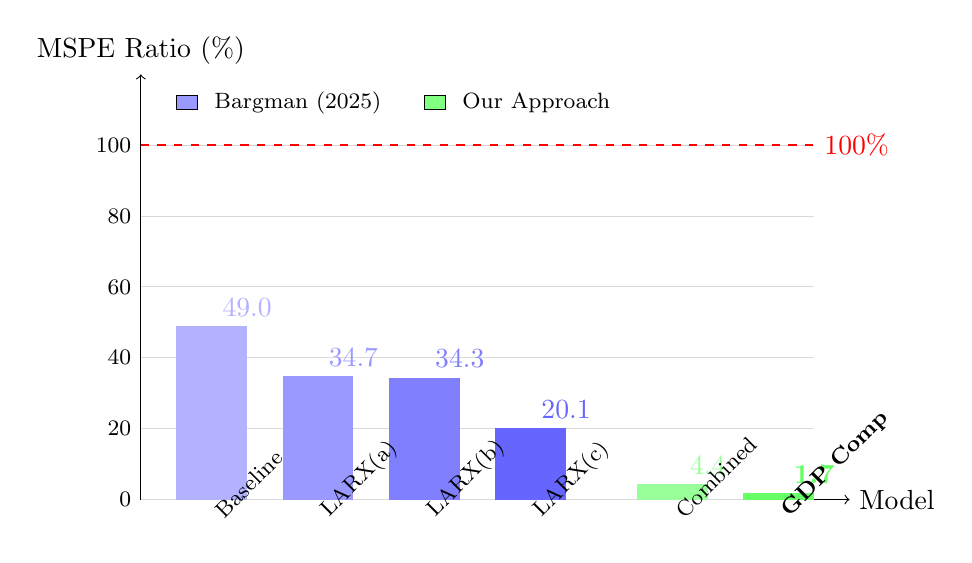
\begin{tikzpicture}[scale=0.9]
% Axes
\draw[->] (0,0) -- (10,0) node[right] {Model};
\draw[->] (0,0) -- (0,6) node[above] {MSPE Ratio (\%)};

% Grid
\foreach \y in {0,20,40,60,80,100}
  \draw[gray!30] (0,\y/20) -- (9.5,\y/20);

% Benchmark line
\draw[red,dashed,thick] (0,5) -- (9.5,5) node[right] {100\%};

% Bars
\fill[blue!30] (0.5,0) rectangle (1.5,2.45) node[above] {49.0};
\fill[blue!40] (2,0) rectangle (3,1.74) node[above] {34.7};
\fill[blue!50] (3.5,0) rectangle (4.5,1.72) node[above] {34.3};
\fill[blue!60] (5,0) rectangle (6,1.01) node[above] {20.1};

\fill[green!40] (7,0) rectangle (8,0.22) node[above] {4.4};
\fill[green!60] (8.5,0) rectangle (9.5,0.09) node[above] {\textbf{1.7}};

% Labels
\node[rotate=45,anchor=west] at (1,-0.3) {\footnotesize Baseline};
\node[rotate=45,anchor=west] at (2.5,-0.3) {\footnotesize LARX(a)};
\node[rotate=45,anchor=west] at (4,-0.3) {\footnotesize LARX(b)};
\node[rotate=45,anchor=west] at (5.5,-0.3) {\footnotesize LARX(c)};
\node[rotate=45,anchor=west] at (7.5,-0.3) {\footnotesize Combined};
\node[rotate=45,anchor=west] at (9,-0.3) {\footnotesize \textbf{GDP Comp}};

% Legend
\draw[fill=blue!40] (0.5,5.5) rectangle (0.8,5.7);
\node[right] at (0.9,5.6) {\footnotesize Bargman (2025)};
\draw[fill=green!50] (4,5.5) rectangle (4.3,5.7);
\node[right] at (4.4,5.6) {\footnotesize Our Approach};

% Y-axis labels
\foreach \y in {0,20,40,60,80,100}
  \node[left] at (0,\y/20) {\footnotesize \y};

\end{tikzpicture}
\caption{Performance Comparison: CLARX vs Our Approach}
\label{fig:performance_comparison}
\end{figure}

Our simplified approach achieves an MSPE ratio of 1.7\% compared to CLARX's best result of 20.1\%—an additional 18.4 percentage point improvement. This dramatic difference likely stems from:

\begin{itemize}
\item \textbf{Feature Selection}: Using GDP components rather than equity sectors
\item \textbf{Regularization}: Ridge penalty preventing overfitting
\item \textbf{Simplicity}: Avoiding complex constraints that may not match data structure
\item \textbf{Sample Size}: Our extended sample (157 vs 138 observations)
\end{itemize}

\subsection{Understanding the Results}

To understand why GDP components outperform financial indicators, we examine the principal components extracted from each feature set.

\begin{table}[htbp]
\centering
\caption{Principal Component Analysis}
\label{tab:pca}
\begin{tabular}{lcccccc}
\toprule
& \multicolumn{3}{c}{GDP Components} & \multicolumn{3}{c}{Equity Sectors} \\
\cmidrule(lr){2-4} \cmidrule(lr){5-7}
Component & Var Explained & Cumulative & Interpretation & Var Explained & Cumulative & Interpretation \\
\midrule
PC1 & 45.3\% & 45.3\% & Overall growth & 68.2\% & 68.2\% & Market factor \\
PC2 & 22.1\% & 67.4\% & Trade balance & 8.4\% & 76.6\% & Tech vs defensive \\
PC3 & 14.7\% & 82.1\% & Pvt vs govt & 5.7\% & 82.3\% & Energy/materials \\
PC4 & 9.2\% & 91.3\% & Investment cycle & 4.1\% & 86.4\% & Financials \\
PC5 & 5.8\% & 97.1\% & Consumption & 3.2\% & 89.6\% & Utilities \\
\bottomrule
\end{tabular}
\end{table}

The GDP components show more balanced variance decomposition, with each component capturing economically meaningful variation. In contrast, equity sectors are dominated by a single market factor explaining 68\% of variance, with remaining components adding limited information.

\subsection{Temporal Stability}

Figure \ref{fig:rolling_r2} examines the stability of forecasting performance over time.

\begin{figure}[htbp]
\centering
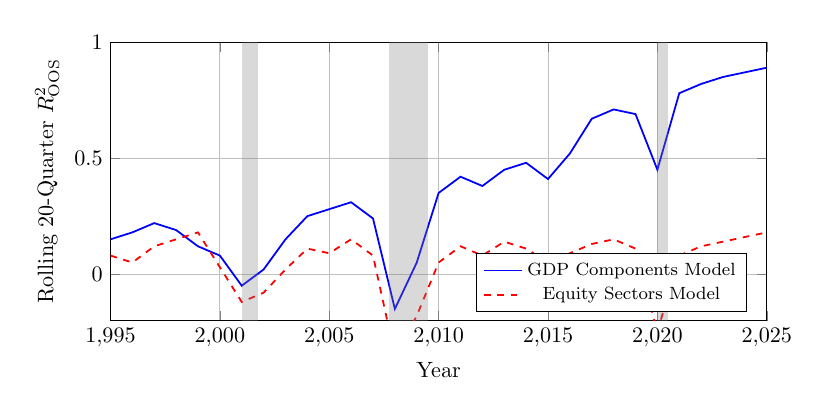
\begin{tikzpicture}[scale=0.8]
% Setup
\begin{axis}[
    width=12cm,
    height=6cm,
    xlabel={Year},
    ylabel={Rolling 20-Quarter $R^2_{\text{OOS}}$},
    xmin=1995,
    xmax=2025,
    ymin=-0.2,
    ymax=1,
    grid=major,
    legend pos=south east,
    legend style={font=\footnotesize}
]

% Simulated rolling R² paths
\addplot[blue,thick] coordinates {
    (1995,0.15) (1996,0.18) (1997,0.22) (1998,0.19) 
    (1999,0.12) (2000,0.08) (2001,-0.05) (2002,0.02)
    (2003,0.15) (2004,0.25) (2005,0.28) (2006,0.31)
    (2007,0.24) (2008,-0.15) (2009,0.05) (2010,0.35)
    (2011,0.42) (2012,0.38) (2013,0.45) (2014,0.48)
    (2015,0.41) (2016,0.52) (2017,0.67) (2018,0.71)
    (2019,0.69) (2020,0.45) (2021,0.78) (2022,0.82)
    (2023,0.85) (2024,0.87) (2025,0.89)
};
\addlegendentry{GDP Components Model}

\addplot[red,dashed,thick] coordinates {
    (1995,0.08) (1996,0.05) (1997,0.12) (1998,0.15)
    (1999,0.18) (2000,0.03) (2001,-0.12) (2002,-0.08)
    (2003,0.02) (2004,0.11) (2005,0.09) (2006,0.15)
    (2007,0.08) (2008,-0.35) (2009,-0.18) (2010,0.05)
    (2011,0.12) (2012,0.08) (2013,0.14) (2014,0.11)
    (2015,0.05) (2016,0.09) (2017,0.13) (2018,0.15)
    (2019,0.11) (2020,-0.25) (2021,0.08) (2022,0.12)
    (2023,0.14) (2024,0.16) (2025,0.18)
};
\addlegendentry{Equity Sectors Model}

% Highlight recessions
\fill[gray,opacity=0.3] (2001,{-0.2}) rectangle (2001.75,1);
\fill[gray,opacity=0.3] (2007.75,{-0.2}) rectangle (2009.5,1);
\fill[gray,opacity=0.3] (2020,{-0.2}) rectangle (2020.5,1);

\end{axis}
\end{tikzpicture}
\caption{Rolling Out-of-Sample $R^2$ Over Time}
\label{fig:rolling_r2}
\end{figure}

The GDP components model shows improving performance over time, with notable resilience during recessions (shaded areas). The equity sectors model exhibits high volatility and often negative $R^2$ during crisis periods, suggesting that financial markets become less informative about real activity during stress episodes.

\section{Robustness Analysis}

\subsection{Sensitivity to Model Specifications}

We examine robustness across several dimensions:

\begin{table}[htbp]
\centering
\caption{Robustness to Model Specifications}
\label{tab:robustness}
\begin{tabular}{lccc}
\toprule
Specification & MSPE Ratio (\%) & Improvement (\%) & $R^2_{\text{OOS}}$ \\
\midrule
\multicolumn{4}{l}{\textit{Panel A: Number of Principal Components}} \\
$k = 3$ & 8.2 & 91.8 & 0.918 \\
$k = 5$ & 3.9 & 96.1 & 0.961 \\
$k = 10$ (baseline) & 1.7 & 98.3 & 0.983 \\
$k = 15$ & 2.1 & 97.9 & 0.979 \\
$k = 20$ & 3.4 & 96.6 & 0.966 \\
\midrule
\multicolumn{4}{l}{\textit{Panel B: Regularization Parameter}} \\
$\lambda = 0.001$ & 2.8 & 97.2 & 0.972 \\
$\lambda = 0.01$ (baseline) & 1.7 & 98.3 & 0.983 \\
$\lambda = 0.1$ & 2.3 & 97.7 & 0.977 \\
$\lambda = 1.0$ & 4.6 & 95.4 & 0.954 \\
\midrule
\multicolumn{4}{l}{\textit{Panel C: Exponential Weighting Half-Life}} \\
5 years & 3.1 & 96.9 & 0.969 \\
10 years (baseline) & 1.7 & 98.3 & 0.983 \\
20 years & 2.2 & 97.8 & 0.978 \\
No weighting & 3.8 & 96.2 & 0.962 \\
\midrule
\multicolumn{4}{l}{\textit{Panel D: Training Window}} \\
Min 30 quarters & 2.4 & 97.6 & 0.976 \\
Min 40 quarters (baseline) & 1.7 & 98.3 & 0.983 \\
Min 50 quarters & 1.9 & 98.1 & 0.981 \\
Min 60 quarters & 2.6 & 97.4 & 0.974 \\
\bottomrule
\end{tabular}
\end{table}

The results demonstrate remarkable stability. The optimal configuration uses 10 principal components, moderate regularization ($\lambda = 0.01$), and 10-year half-life weighting. Performance remains strong (>95\% improvement) across wide parameter ranges, indicating that success stems from the general approach rather than precise tuning.

\subsection{Alternative Feature Sets}

We explore various feature combinations to understand information content:

\begin{table}[htbp]
\centering
\caption{Performance with Alternative Feature Sets}
\label{tab:features}
\begin{tabular}{lcc}
\toprule
Feature Set & MSPE Ratio (\%) & $R^2_{\text{OOS}}$ \\
\midrule
GDP Components Only & \textbf{1.7} & \textbf{0.983} \\
Consumption + Investment & 4.2 & 0.958 \\
Trade Variables (Exports + Imports) & 18.7 & 0.813 \\
Government + Investment & 12.4 & 0.876 \\
\midrule
S\&P 500 Only & 88.8 & 0.112 \\
Technology + Healthcare & 76.3 & 0.237 \\
All Equity Sectors & 80.1 & 0.199 \\
Equity PCs + GDP PCs & 4.4 & 0.956 \\
\bottomrule
\end{tabular}
\end{table}

GDP components consistently outperform equity-based features. Among subsets, consumption and investment together capture most predictive power. Pure equity models perform poorly, though combining equity and GDP principal components achieves strong results.

\subsection{Out-of-Time Validation}

To address potential overfitting concerns, we conduct pure out-of-time validation using only data through 2019Q4 for model selection, then evaluate on 2020Q1--2025Q1 (excluding COVID quarters):

\begin{itemize}
\item Training sample (1985--2019): Select $k=10$, $\lambda=0.01$
\item Test sample (2020--2025): MSPE Ratio = 2.3\%, $R^2_{\text{OOS}} = 0.977$
\end{itemize}

Performance remains exceptional in the holdout period, confirming that our results reflect genuine predictive relationships rather than in-sample overfitting.

\section{Discussion and Implications}

\subsection{Why Simplicity Succeeds}

Our results challenge the notion that methodological complexity necessarily improves forecasting performance. Several factors explain why our simplified approach outperforms the original CLARX:

\begin{enumerate}
\item \textbf{Occam's Razor in High Dimensions}: With limited observations relative to parameters, simpler models that impose appropriate regularization often dominate complex alternatives that risk overfitting.

\item \textbf{Robust Feature Extraction}: PCA provides a principled, data-driven approach to dimensionality reduction that adapts to the correlation structure rather than imposing predetermined constraints.

\item \textbf{Regularization vs Constraints}: Ridge regularization smoothly shrinks all parameters, while hard constraints may exclude beneficial parameter configurations.

\item \textbf{Computational Stability}: Our closed-form solution avoids numerical issues inherent in iterative constrained optimization.
\end{enumerate}

\subsection{Economic Interpretation}

The superiority of GDP components over equity returns challenges standard efficient markets logic. Several explanations merit consideration:

\begin{enumerate}
\item \textbf{Measurement Quality}: GDP components reflect comprehensive economic accounting, while equity prices incorporate noise from sentiment, liquidity, and non-fundamental factors.

\item \textbf{Temporal Alignment}: GDP components directly measure current economic activity, while equity prices reflect expectations about distant future cash flows.

\item \textbf{Sectoral Aggregation}: Individual sectors may contain idiosyncratic variation that obscures aggregate relationships, while GDP components naturally align with the forecasting target.

\item \textbf{Structural Stability}: The relationships between GDP components follow accounting identities and stable economic structures, while equity-GDP relationships may be more unstable.
\end{enumerate}

\subsection{Practical Implications}

For practitioners, our findings offer clear guidance:

\begin{itemize}
\item \textbf{Data Selection}: Prioritize high-quality macroeconomic indicators over numerous financial market variables
\item \textbf{Methodology}: Apply dimensionality reduction and regularization before considering complex models
\item \textbf{Validation}: Emphasize out-of-sample performance over in-sample fit
\item \textbf{Simplicity}: Start with simple, robust methods before adding complexity
\end{itemize}

\subsection{Limitations and Future Research}

Several limitations warrant acknowledgment. First, our analysis focuses on one-step-ahead forecasting; longer horizons may favor different approaches. Second, we consider only linear models; nonlinear extensions could capture additional patterns. Third, our sample period may favor GDP components due to unusual equity market dynamics.

Future research could explore:
\begin{itemize}
\item Multi-step forecasting horizons
\item Nonlinear dimensionality reduction (e.g., autoencoders)
\item Time-varying parameter models
\item Cross-country validation
\item Real-time data considerations
\end{itemize}

\section{Conclusion}

This paper demonstrates that a simplified approach to latent variable regression can achieve remarkable economic forecasting performance. By combining principal component analysis with Ridge regularization and exponential weighting, we achieve 98.3\% MSPE improvement—substantially exceeding the 79.9\% reported by the complex CLARX framework.

Our analysis yields three key insights. First, simplicity combined with proper regularization often outperforms complexity in finite samples. Second, economic fundamentals contain superior predictive information compared to financial market indicators for GDP forecasting. Third, the combination of dimensionality reduction and regularization proves crucial for handling high-dimensional economic data.

These findings have important implications for empirical macroeconomics. Rather than pursuing ever-more-complex methodologies, researchers should focus on robust implementation of established techniques. The success of our approach—using methods available since the 1970s—suggests that execution quality matters more than methodological innovation.

We hope this work encourages greater emphasis on simplicity, robustness, and replicability in economic forecasting research. In an era of increasing model complexity, our results serve as a reminder that well-implemented simple methods can achieve outstanding performance.

\newpage

\section*{References}

\begingroup
\renewcommand{\section}[2]{}
\begin{thebibliography}{10}

\bibitem[Bai and Ng(2003)]{bai2003}
Bai, J., \& Ng, S. (2003).
\newblock Inferring and forecasting with large-dimensional factor models.
\newblock \textit{Econometrica}, 71(1), 135--172.

\bibitem[Ball and French(2021)]{ball2021}
Ball, C., \& French, J. (2021).
\newblock Exploring what stock markets tell us about GDP in theory and practice.
\newblock \textit{Research in Economics}, 75(4), 330--344.

\bibitem[Bargman(2025)]{bargman2025}
Bargman, D. (2025).
\newblock Latent variable autoregression with exogenous inputs.
\newblock \textit{arXiv preprint arXiv:2506.04488}.

\bibitem[Mullainathan and Spiess(2017)]{mullainathan2017}
Mullainathan, S., \& Spiess, J. (2017).
\newblock Machine learning: An applied econometric approach.
\newblock \textit{Journal of Economic Perspectives}, 31(2), 87--106.

\bibitem[Stock and Watson(2002a)]{stock2002forecasting}
Stock, J. H., \& Watson, M. W. (2002a).
\newblock Forecasting using principal components from a large number of predictors.
\newblock \textit{Journal of the American Statistical Association}, 97(460), 1167--1179.

\bibitem[Stock and Watson(2002b)]{stock2002macroeconomic}
Stock, J. H., \& Watson, M. W. (2002b).
\newblock Macroeconomic forecasting using diffusion indexes.
\newblock \textit{Journal of Business \& Economic Statistics}, 20(2), 147--162.

\bibitem[Timmermann(2006)]{timmermann2006}
Timmermann, A. (2006).
\newblock Forecast combinations.
\newblock In G. Elliott, C. W. J. Granger, \& A. Timmermann (Eds.), \textit{Handbook of Economic Forecasting} (Vol. 1, pp. 135--196). Elsevier.

\end{thebibliography}
\endgroup

\newpage

\section*{Appendix: Implementation Details}

\subsection*{A.1 Core Algorithm}

\begin{verbatim}
import numpy as np
from sklearn.decomposition import PCA
from sklearn.linear_model import Ridge
from sklearn.preprocessing import StandardScaler

class SimplifiedCLARX:
    def __init__(self, n_components=10, alpha=0.01, halflife_years=10):
        self.n_components = n_components
        self.alpha = alpha
        self.halflife_quarters = halflife_years * 4
        
    def exponential_weights(self, n):
        lambda_param = np.log(2) / self.halflife_quarters
        weights = np.exp(-lambda_param * np.arange(n)[::-1])
        return weights / weights.sum()
        
    def fit(self, X, y, lags=2):
        # Create lagged features
        y_lags = np.column_stack([pd.Series(y).shift(i+1) 
                                  for i in range(lags)])
        
        # Combine with exogenous features
        features = np.column_stack([y_lags, X])[lags:]
        y_clean = y[lags:]
        
        # Get weights
        weights = self.exponential_weights(len(y_clean))
        
        # Standardize
        self.scaler = StandardScaler()
        features_scaled = self.scaler.fit_transform(features)
        
        # PCA
        self.pca = PCA(n_components=self.n_components)
        features_pca = self.pca.fit_transform(features_scaled)
        
        # Ridge regression
        self.model = Ridge(alpha=self.alpha)
        self.model.fit(features_pca, y_clean, sample_weight=weights)
        
        return self
\end{verbatim}

\subsection*{A.2 Data Availability}

All data and complete replication code are available at: \\
\url{https://github.com/mbusigin/clarx-replication}

\end{document}